% This is main.tex, a sample paper demonstrating the use of the
% LLNCS macro package for Springer Computer Science proceedings;
% Version 2.20 of 2017/10/04
% 
\documentclass[runningheads]{llncs}
%
% ---- Packages ----
%
\usepackage{graphicx} % enhanced support for graphics
\usepackage{url} % add macros for handling URLs in text
\usepackage[nohyperlinks,nolist]{acronym} % abbreviation utilities
\usepackage{listings}
\usepackage{hyperref}



% Capitalize autoref{..}
\def\chapterautorefname{Chapter}
\def\sectionautorefname{Section}
\def\subsectionautorefname{Subsection}
\def\algorithmautorefname{Algorithm}
\def\subfigureautorefname{Figure}
\def\itemautorefname{Step}
%
% ---- Acronyms ----
%
\begin{acronym}
\acro{rq}[RQ]{Research Question}
\end{acronym}
%
% ---- Begin Document ----
%
\begin{document}
%
\title{Evaluating Code Clone Frequency In Different-Generation Programming Languages}
%
%\titlerunning{Abbreviated paper title}
% If the paper title is too long for the running head, you can set
% an abbreviated paper title here
%
% ---- Author Information ----
%
\author{Jonas Schuhmacher, Jakob Rott}
\institute{Seminar: Software Quality (SS2022)\\
Technical University of Munich\\
\email{jonas.schuhmacher@tum.de, rott@cqse.eu}}
%
\maketitle % typeset the header of the contribution
%
% ---- Abstract ----
%
\begin{abstract}
The abstract should briefly summarize the contents of the paper in
15--250 words.

\keywords{First keyword  \and Second keyword \and Another keyword.}
\end{abstract}
%
% ---- Text Parts ----
%
\section{Introduction}
\label{sec:intro}

\subsection{Motivation}
\label{sec:intro:sub:motivation}

Please note that the first paragraph of a section or subsection is not indented.
The first paragraph that follows a table, figure, equation etc. does not need an indent, either.\footnote{Here is a sample footnote with a URL: \url{http://google.com}}

Subsequent paragraphs, however, are indented.

\subsubsection{Sample Heading (Third Level)} Only two levels of
headings should be numbered. Lower level headings remain unnumbered; they are formatted as run-in headings.

\paragraph{Sample Heading (Fourth Level)}
The contribution should contain no more than four levels of headings. 
Table~\ref{tab1} gives a summary of different text styles.

\begin{table}
\caption{Table captions should be placed above the
tables.}\label{tab1}
\centering
\begin{tabular}{|l|l|l|}
\hline
First col &  Second col & Third col\\
\hline
Normal & \textbf{Bold} & \textit{Italique}\\
\texttt{Typewriter} & \textsc{small caps} & \underline{underline}\\
\hline
\end{tabular}
\end{table}


\noindent Displayed equations are centered and set on a separate
line.
\begin{equation}
x + y = z
\end{equation}
Please try to avoid rasterized images for line-art diagrams and schemas. 
Whenever possible, use vector graphics instead (see Fig.~\ref{fig1}).

\begin{figure}
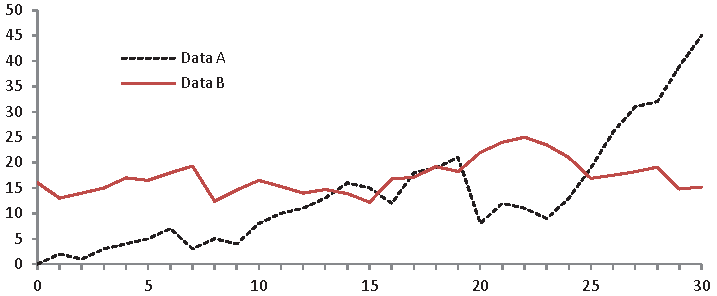
\includegraphics[width=\textwidth]{figures/fig1}
\caption{A figure caption is always placed below the illustration.
Please note that short captions are centered, while long ones are justified by the macro package automatically.} 
\label{fig1}
\end{figure}

\begin{theorem}
This is a sample theorem. 
The run-in heading is set in bold, while the following text appears in italics. 
Definitions, lemmas, propositions, and corollaries are styled the same way.
\end{theorem}
%
% the environments 'definition', 'lemma', 'proposition', 'corollary',
% 'remark', and 'example' are defined in the LLNCS documentclass as well.
%
\begin{proof}
Proofs, examples, and remarks have the initial word in italics, while the following text appears in normal font.
\end{proof}
For citations of references, we prefer the use of square brackets and consecutive numbers. 
Citations using labels or the author/year convention are also acceptable. 
The following bibliography provides a sample reference list with entries for journal articles~\cite{Stol2016}, a book~\cite{Myers2012}, conference proceedings~\cite{Harrold1988}, and a web site~\cite{Schaffer2018}.

\subsection{Abbreviations}
\label{sec:intro:sub:abbrev}

To use acronyms in the document, simple declare them in the main.tex file and use them later.
For example, you might want to define \acp{rq}, which will then be always abbreviated as \ac{rq} for singular or \acp{rq} for plural.

List are also really easy to create:

\begin{itemize}
  \item One entry in the list
  \item Another entry in the list
\end{itemize}

\begin{enumerate}
  \item The labels consists of sequential numbers.
  \item The numbers starts at 1 with every call to the enumerate environment.
\end{enumerate}

\subsection{Code Listings}
\label{sec:intro:sub:code}

Listings can either be created inside the text or imported:\footnote{See \url{https://www.overleaf.com/learn/latex/Code_listing} for a complete example.}
\begin{lstlisting}[language=C]
int main(int argc, char* argv[]) {
  return 0;
}
\end{lstlisting}
% !TeX spellcheck = en_US

\section{Related Work}
\label{sec:related_work}

In general, we can subdivide this section in two categories. First, existing works searching for the reasons for code clones in human, organizational and technological factors are examined and secondly, we focus on papers describing explicitly the correlation between certain languages and the appearance of code clones.

\subsection{Reasons for Code Clones}
\label{sec:reasons_for_code_clones}

\subsubsection{Human \& Organizational Factors}

Before describing how the choice of programming language can affect clones, we start with a brief overview on other reasons for clones. Here, first to mention are human factors like inadvertently or impatiently copying because time or understanding are missing. Missing abstraction and contrary the need to fulfill certain coupling and cohesion properties are also potential sources of generating code clones \cite{kasper2006cloning}.
The intention to minimize the risks when adopting new ideas in software are also driver for cloning code since this technique allows to keep errors through the introduced redundancy in just a single module \cite{cordy2003comprehending}. Further as time-to-market is critical, cloning can improve the speed of developing an early prototype, as analyzed by \cite{rajapakse2007using} for web-applications.

\subsubsection{Technological Factors}

Alongside these human and economic factors are standing "[t]echnology limitations" \cite{kasper2006cloning} like the utilization of a specific programming language.
\textit{Templating} is major feature of modern programming languages like \texttt{C++}, in contrast languages like \texttt{C} do not offer any equivalent feature. Given a certain algorithm working with double precision in the \texttt{C} programming language, the developer is forced to copy the procedure and replace "\texttt{double}" with "\texttt{float}". Such "boiler-plating [is enforced only] due to language inexpressiveness" \cite{kasper2006cloning}. 
Next to those more direct issues with Templating/ generalization in certain languages are keywords, standard library, and patterns how to fulfill certain tasks. For example, creating a \texttt{socket} and communicating with it varies and is different in each programming language - sometimes shorter, sometimes more lengthy, but usual there is one optimal way of doing it, so that possible exception (if the languages even has such a feature) or error codes are handled. These optimal sequences will then be often copy-and-pasted by developers \cite{kasper2006cloning}.
Further next to \textit{templating}, Kasper et. al. \cite{kasper2006cloning} mentions \textit{customization} as reasons for duplication. Code ownership can make bug fixing difficult, only allowing the creation of a work-around by copying and improving the faulty lines. Further, they number the idiom of "replicate and specialize", in which developers clone code to specialize a solution rather than generalizing an existing an implementation.
Lastly, Kasper et. al. \cite{kasper2006cloning} describe \textit{exact matches}, in context of code clones, as a result of copying "semantic properties [of] otherwise unrelated functionality" \cite{kasper2006cloning} between methods like logging or debugging statements and reusing certain code structures like loops which are easier copied than implemented as reusable function.

\subsection{Similar Analyses}
\label{sec:similiar_analyses}

This work will later present a comparison of clone coverage in different generation programming languages, but there are already some studies with a similar scope.

\subsubsection{Code Clones in Build Systems}

Once developer produced the different components of a large-scale software system, they typically need to be assembled together. This critical step usually accomplished with certain build systems like \texttt{Ant}, \texttt{Maven}, \texttt{Autotools} or \texttt{CMake} for respectively \texttt{Java} and \texttt{C/C++}. \cite{mcintosh2014collecting} compares these build systems with surprising results. As overall result, "build systems tend to have higher cloning rates than other software artifacts" \cite{mcintosh2014collecting}. 
They conclude with the finding that, as opposed of what one might think, modern build systems like \texttt{CMake} and \texttt{Maven} have higher clone coverage then their older counterparts and the \texttt{C/C++} systems and vice-versa \texttt{Java} build systems have a higher clone coverage, in many cases more than $50\%$, than the respective \texttt{C/C++} counterparts.

\subsubsection{Comparison of Java \& Scala}

Jorge et. al. \cite{jorge2012impact} directly compares features of the two languages \texttt{Java} and \texttt{Scala} and studies how their language constructs correlate to code cloning. In their findings, they conclude that code duplication problems arise with higher probability if a language is more verbose, e.g. due to getters and setters, anonymous classes, constructors, and lacks (simple) abstraction capabilities. Properties which finally lead to more effort refactoring code than simply cloning a source code. \cite{jorge2012impact}

\section{Methodology}
\label{sec:methodology}

Present the UML structure of the analysis, as well as the selection criterion/ sources.
\section{Results}
\label{sec:results}

Present the plots and give some rough description of on them
\section{Discussion}
\label{sec:discussion}

Confirm the thesis.
\section{Conclusion}
\label{sec:conclusion}

Summarize and give outlook

%
% ---- Appendix ----
%
\appendix
\section{Appendix}
\label{sec:appendix}

Anything additional goes here \dots
%
% ---- Bibliography ----
%
\bibliographystyle{splncs04}
\bibliography{library}
%
\end{document}
%
% ---- Begin Document ----
%
